\documentclass[main.tex]{subfiles}

\begin{document}

\subsection{Adaptation code}
In this section, the adaptation code is described that was written to execute the test suites generated by the MTR tool for the Kubernetes pod lifecycle model. The purpose of the adaptation code is to interface with the Kubernetes cluster using `kubectl ` commands and to monitor pod states based on the inputs from the test suite and the expected results.

To parse the generated test suites, a JSON test suite parser was written. It returns the input and the output symbols in a list, so that the test runner class can easily iterate through them and execute each transition. 
The adaptation code contains two important mappings, which also contain the main logic of the program:
\begin{itemize}
\item \textbf{Input Mappers}: The input mapper maps the current input symbol to the corresponding function call in the program. This is where it is decided which Kubernetes action needs to be taken (e.g., creating or deleting a Pod). The input is mapped to the relevant functions that handle the Kubernetes API interactions through `kubectl`. Each transition was performed with \texttt{kubectl apply -f} command, where different Pod definitions were provided for the different test scenarios. For example to test a Pod getting into the ImagePullBackOff state, the Pod definition intentionally contained a faulty image name. 

\textit{Notes on limitations: Since it is not permitted by the Kubernetes API to modify certain properties of a Pod such as Liveness probes while running, it was only possible to carry out each transitions if every time the Pod was deleted and then recreated with a new Pod definition. This actually caused longer runtime, especially because before some actions like asserting that the pull of a Docker image was successfull it was necessary to include some waiting times.} 

\item \textbf{Output Mappers}: Since the FSM model was created in a way that the output symbols correspond to the next state of the model, these could be used for assertions too. For this, the output mapper translates the states into assertions, where we check the Pod states after each transitions. So in the end, the result of these checks are compared to the current expected output symbol of the generated test suite.
\end{itemize}

In summary, the adaptation code works as follows:
\begin{itemize}
    \item \textbf{Test Suite Parsing}: The test suite JSON is parsed to extract the input and expected output list.
    \item \textbf{Kubernetes Interaction}: Using `kubectl`, the code performs the corresponding actions (e.g., creating a Pod with different definitions, deleting a Pod).
    \item \textbf{State Monitoring}: The code monitors the pod's state after each operation and compares it against the expected output.
\end{itemize}

\subsection{Example use case: successful Pod deployment}
In this section, we go into the implementation details of our adaptation code by illustrating a practical use case: a Kubernetes Pod being successfully created, the containers are running, then transitioning to the Running state, and subsequently being deleted. 

Precondition: any Kubernetes cluster is running, in our case it is Minikube, and in the default namespace, there is no Pod with the same name as we want to use.

To create a test Pod in the Java project, under the source/main/resources there is a Pod resource file test-pod.yaml. This YAML file is applied by kubectl command to deploy the target pod:

\begin{lstlisting}[language=yaml]
apiVersion: v1
kind: Pod
metadata:
  name: test-pod
spec:
  terminationGracePeriodSeconds: 2
  containers:
    - name: nginx
      image: nginx
      ports:
        - containerPort: 80
      livenessProbe:
        exec:
          command:
            - "true"
        initialDelaySeconds: 2
        periodSeconds: 2
      readinessProbe:
        exec:
          command:
            - "true"
        initialDelaySeconds: 5
        periodSeconds: 2
  restartPolicy: Never
\end{lstlisting}

To simulate and test this specific use case, there is a Example\_Use\_Case1-test\_suite.json test suite JSON file under source/main/resources/test\_suites folder with the necessary input/output list. This suite file is parsed by the executed test program, and based on the input list, the output of the deployed pod is verified. The test case is successful only if all input/output pairs are verified:

\begin{lstlisting}[language=json]
{
    "test_suite": {
        "name": "Example_Use_Case1",
        "id": "d4b3d5c2-8e4e-4b47-a36b-b2f7aab7e7d6",
        "method": "Custom",
        "input_list": [
            "create_pod",
            "image_pull_success",
            "containers_ready",
            "rediness_probe_success",
            "delete_pod",
            "clean_up"
        ],
        "output_list": [
            "Pending",
            "ContainerCreating",
            "Running_NotReady",
            "Running_Ready",
            "Terminating",
            "PodNotExists"
        ]
    }
}\end{lstlisting}
\vspace{10pt}

This is the current entry point of the program:
\begin{lstlisting}[language=Java]
package test_runners;

import utils.JsonTestSuiteProcessor;
import utils.TestSuite;
import utils.Utils;

public class ExampleUseCase1TestRunner {

    public static void main(String[] args) throws Exception {
        TestSuite testSuite = JsonTestSuiteProcessor.loadTestSuite(Utils.getResourceFilePath("test_suites/Example_Use_Case1-test_suite.json")).testSuite;
        TestRunner testRunner = new TestRunner();
        testRunner.runTestSuite(testSuite);
    }
}
\end{lstlisting}

The above test suite json is parsed and executed by TestRunner.runTestSuite method. This method loops through the input list and verifies the Pod state provided by output element in the output list.

\begin{lstlisting}[language=Java]
public void runTestSuite(TestSuite testSuite) throws FileNotFoundException, URISyntaxException, InterruptedException {
        long startTime = System.currentTimeMillis();
        boolean allTestPassed = true;
        boolean currentResult;

        KubectlUtils.deletePod("test-pod"); // fresh start

        List<String> inputs = testSuite.getInputList();
        List<String> expectedOutputs = testSuite.getOutputList();
        int testSuiteLength = inputs.size();

        // Iterate through all test cases
        for (int i = 0; i < testSuiteLength; i++) {
            String input = inputs.get(i);
            String expectedOutput = expectedOutputs.get(i);

            // Execute the corresponding InputExecutor for the given input
            if (inputFunctionMap.containsKey(input) && outputMap.containsKey(expectedOutput)) {
                System.out.println(STR."Running test for input: \{input}");
                System.out.println(STR."Expected output: \{expectedOutput}");
                currentResult = Utils.processInput(inputFunctionMap.get(input), outputMap.get(expectedOutput));
            } else {
                throw new IllegalArgumentException(STR."Unknown input: \{input}");
            }

            if (currentResult) {
                System.out.println("--------------------------------------------------");
                System.out.println(STR."Test (\{i+1}/\{testSuiteLength}) passed for input: \{input}");
                System.out.println("--------------------------------------------------");
            } else {
                System.out.println("--------------------------------------------------");
                System.out.println(STR."Test (\{i+1}/\{testSuiteLength}) failed for input: \{input}");
                System.out.println(STR."Expected: \{expectedOutput}");
                System.out.println("--------------------------------------------------");
            }

            allTestPassed = allTestPassed && currentResult;
        }

        long endTime = System.currentTimeMillis();
        System.out.println("\n");
        System.out.println(STR."Elapsed time: \{(endTime-startTime)/1000} s");
        if (allTestPassed) {
            System.out.println("All test passed!\n\n");
        } else {
            System.out.println("There were failures...\n\n");
        }
    }

\end{lstlisting}

All input elements are mapped to an InputExecutor instance and all output elements are mapped to an OutputMapper instance, and each input and output element has its own implementation.

\begin{lstlisting}[language=Java]
static {
        // Map input commands to their respective InputExecutor implementations
        inputFunctionMap.put("create_pod", new PodCreateInputExecutor());
        inputFunctionMap.put("image_pull_success", new ImagePullSuccessInputExecutor());
        inputFunctionMap.put("delete_pod", new DeletePodInputExecutor());
        inputFunctionMap.put("clean_up", new CleanUpInputExecutor());
        inputFunctionMap.put("image_pull_error", new ImagePullErrorInputExecutor());
        inputFunctionMap.put("containers_ready", new ContainersReadyInputExecutor());
        inputFunctionMap.put("rediness_probe_success", new ReadinessProbeSuccessInputExecutor());
        inputFunctionMap.put("rediness_probe_failure", new ReadinessProbeFailureInputExecutor());
        inputFunctionMap.put("one_container_failed", new OneContainerFailedInputExecutor());
        inputFunctionMap.put("container_terminated", new ContainerTerminatedInputExecutor());
        inputFunctionMap.put("timeout", new TimeoutInputExecutor());
        inputFunctionMap.put("containers_exited_succ", new ContainersExitedSuccessInputExecutor());
        inputFunctionMap.put("check_status", new CheckStatusInputExecutor());

        // Map output states to their respective OutputMapper implementations
        outputMap.put("ContainerCreating", new ContainerCreatingOutputMapper());
        outputMap.put("CrashLoopBackOff", new CrashLoopBackOffOutputMapper());
        outputMap.put("Failed", new FailedOutputMapper());
        outputMap.put("ImagePullBackOff", new ImagePullBackOffOutputMapper());
        outputMap.put("Pending", new PendingOutputMapper());
        outputMap.put("PodNotExists", new PodNotExistsOutputMapper());
        outputMap.put("Running_NotReady", new RunningNotReadyOutputMapper());
        outputMap.put("Running_Ready", new RunningReadyOutputMapper());
        outputMap.put("Succeeded", new SucceededOutputMapper());
        outputMap.put("Terminating", new TerminatingOutputMapper());
        outputMap.put("", new PodNotExistsOutputMapper());
    }
\end{lstlisting}

An input/output pair is validated by Utils.processInput static method which returns true if the expected output matches the actual state of the Pod after the input is processed and executed: 

\begin{lstlisting}[language=Java]
public static boolean processInput(InputExecutor inputExecutor, OutputMapper expectedOutput) throws FileNotFoundException, URISyntaxException, InterruptedException {
        return inputExecutor.execute(expectedOutput);
    }    
\end{lstlisting}

The console output of the example test run:

\begin{figure}[H]
    \centering
    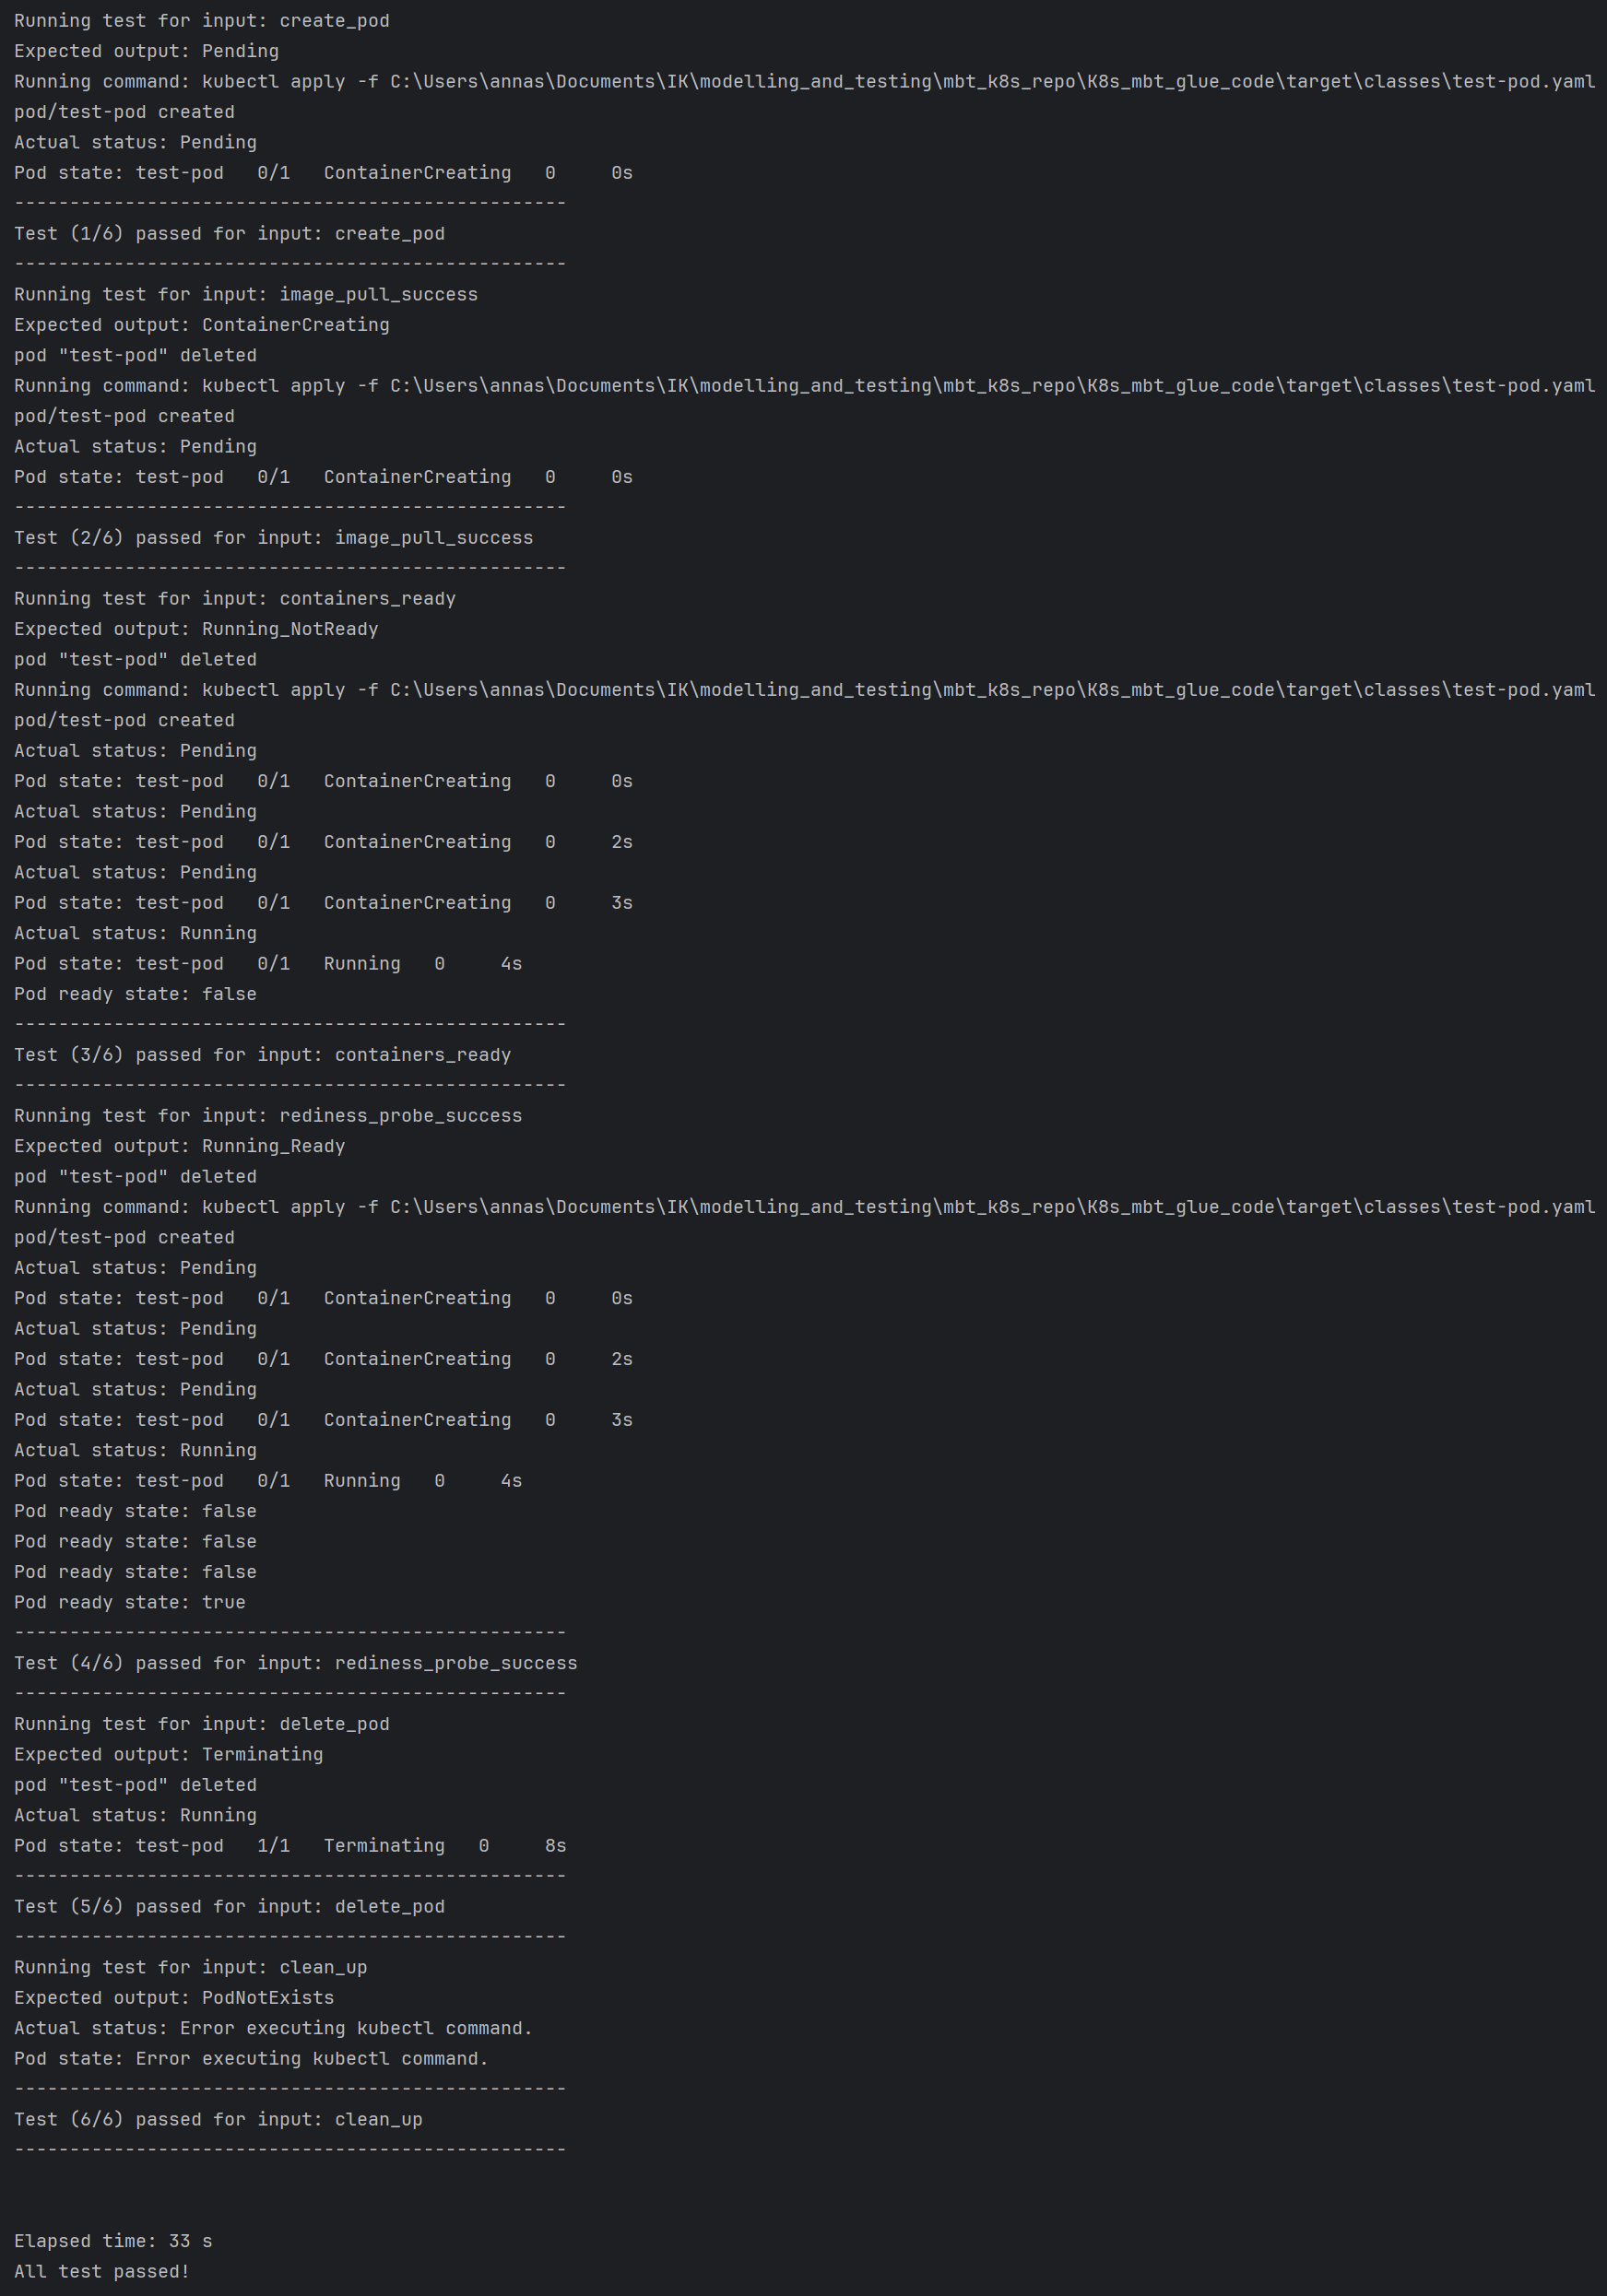
\includegraphics[height=0.85\paperheight,width=\textwidth]{test_results/Example_Use_Case1_testrun.png}
    \caption{Example Use Case1 test result}
    \label{fig:example}

\end{figure}

\subsection{Prerequisites}
The adaptation code was developed and executed on a Windows machine with the following setup:

\begin{itemize}
    \item \textbf{Docker Desktop}: Version 4.19.0 (or the latest version available) - used for running a local Kubernetes cluster in conjunction with Minikube.
    \item \textbf{Minikube}: Version 1.30.0 (or the latest version available) - used to create and manage a local Kubernetes cluster.
    \item \textbf{kubectl}: Version 1.25.0 (or the latest version available) - the Kubernetes command-line tool used to interact with the Kubernetes API for managing pods, deployments, etc.
    \item \textbf{Java}: Version 17 (or the most recent version of the OpenJDK) - the programming language used for writing the adaptation code and handling the test execution.
\end{itemize}
For being able to run the test, the above mentioned tools are needed, and the Docker Desktop and Minikube must be started.

\subsection{Test Execution Report}
The test execution phase was carried out using the adaptation code, which interfaces with the Kubernetes cluster and executedthe generated test suites. The results of these executions, including any errors or issues encountered, are summarized in the following sections.

All of the test suites were executed that was generated by the algorithms described in the previous chapter:
Random walk (100\% state coverage), All State, Transition Tour, Directed Chinese Postman, All Transition State, N-switch coverage. Neither of them discovered any fault, all test passed. The differences were only the test execution times, which were expected because of the various test sequence lengths. Furthermore, as mentioned above, some transitions like Docker image pull, or waiting for a Pod to become ready required more waiting time, so the test suite that used more of these types of transitions were naturally longer to execute.
The following table summarizes the execution times:
\begin{table}[h!]
\centering
\begin{tabular}{|l|c|c|c|}
\hline
\textbf{Algorithm}     & \textbf{Elapsed Time} & \textbf{Test sequence length}\\ \hline
Random Walk (100\% state c.)     & 232 s & 34 \\ \hline
All-State     & 141 s & 18 \\ \hline
Transition Tour     & 330 s    & 54 \\ \hline
DCP     & 299 s    & 54 \\ \hline
All-Transition-State     & 1510 s  & 193\\ \hline
N-Switch Coverage (N=1)     &  1523 s   &  200 \\ \hline
\end{tabular}
\caption{Comparison of Test Executions}
\label{tab:test_exec_comparison}
\end{table}

\subsection{Conclusion}
Based on the results of the test executions, we conclude that the Kubernetes pod lifecycle management is functioning as expected. All test cases passed, and no issues were identified during the testing phase.

\end{document}